\documentclass[25pt, a0paper, portrait]{tikzposter}
\title{\parbox{\linewidth}{\centering Bayesian Non-Parametric Inference
                        in Multivariate Peaks-over-Thresholds Models}}
\author{Peter Trubey}
\date{September 7, 2022}
\institute{UC Santa Cruz; Department of Statistics}

\usepackage{blindtext}
\usepackage{amsmath}
\usepackage{amssymb}
\usepackage{bm}
\usepackage{comment}

\usetheme{Board}

\begin{document}

\maketitle

\block{~}
{
    \blindtext
}

\begin{columns}
    \column{0.5}
    \block{Multivariate Peaks-over-Thresholds}{
        Consider a $d$-dimensional random vector $\bm{W} = (W_1,\ldots,W_d)$ with cumulative distribution function $F$.  
        Assume the existence of sequences of vectors $\bm{a}_n,\bm{b}_n$ such that 
        \[\lim\limits_{n\to\infty}F^n\left(\bm{a}_n\bm{w} + \bm{b}_n\right) = G(\bm{w}),\] 
        then $G$ is a $d$-variate 
        generalized extreme value distribution.  It follows that
        \[
        \lim\limits_{n\to\infty}\text{Pr}\left(\frac{\bm{W} - \bm{b}_n}{\bm{a}_n} \leq \bm{w}\mid \bm{W} 
            \not\leq \bm{b}_n\right) = \frac{\log G(\bm{w}\wedge \bm{0}) - \log G(\bm{w})}{\log G(\bm{0})} = H(\bm{w}),
            \]
        where $H$ is the multivariate Pareto distribution.  That is, excesses \emph{over} the threshold 
        $b = \lim\limits_{n\to\infty} \bm{b}_n$ will be multivariate Pareto.  This comprises the cornerstone of 
        \emph{peaks over threshold} modelling.  In practice, we take a sufficiently large threshold $\bm{b}$, and model
        excesses over that threshold as generalized Pareto.
        
        For ease of interpretation, we transform $W$ to standardized marginals. Let 
        \[Z_{\ell} = \left(1 + \xi_{\ell}\frac{w_{\ell} - b_{\ell}}{a_{\ell}}\right))+^{1/\xi_{\ell}},\]
        then $\bm{Z}$ follows the standard multivariate Pareto distribution.  Remark 3.1 of \cite{rootzen2018} shows how
        we can factorize \[\bm{Z} = R\bm{V},\;\;R\in\mathbb{R}_+;\;V\in\mathbb{S}_{\infty}^{d-1},\] with $R$ independent
        of $\bm{V}$. That is, we can factorize $Z$ into \emph{independent} angular and radial components. $R$ will follow
        a standard Pareto distribution, and $\bm{V}$ will be 
        
        
        will contain all information related to the dependence structure of $\bm{W}$ in extreme regions.  
        For that reason, we seek a flexible distribution to model $\bm{V}$.
        }
    
    \column{0.5}
    \block{Angular Space}{
        We recognize $\mathbb{S}_{\infty}^{d-1}$ as the positive orthant of the unit hypersphere, under the 
        $\mathcal{L}_{\infty}$ norm.  If we consider the $\mathcal{L}_p$ norm, and then the $\mathbb{L}_{\infty}$ norm is expressed as the limit of the $\mathcal{L}_p$ norm,
        \[
            \lVert \bm{s}\rVert_p = \left(\sum_{\ell = 1}^d s_{\ell}^p\right)^{1/p},\;\;\;
            \lVert \bm{s}\rVert_{\infty} = \lim\limits_{p\to\infty}\lVert \bm{s}\rVert_p = \bigvee_{\ell = 1}^d \bm{s}.\]
        If we define $\mathbb{S}_{\infty}^{d-1}$ using this norm, then we consider it the limit of of an expanding 
        series of manifolds $\mathbb{S}_p^{d-1}$, the positive orthant of the unit hypersphere under the $\mathcal{L}_p$ 
        norm.  That is, for $\bm{s}\in R_+^d$,
        \[ \mathbb{S}_{\infty}^{d-1} = \lim\limits_{p\to\infty}\left\lbrace \bm{x}\;\lVert \bm{x}\rVert_p = 1\right\rbrace.\]
        To establish a distribution on $\mathbb{S}_p^{d-1}$, we project a random vector from 
        $\mathbb{R}_+^d$ onto $\mathbb{S}_p^{d-1}$.  That is, for $\mathbb{x}\in\mathbb{R}_+^d$, let 
        $\bm{y} = \frac{\bm{x}}{\lVert\bm{x}\rVert_p} \in \mathbb{S}_p^{d-1}$.  Then, by letting 
        $y_d = \left(1 - \sum_{\ell = 1}^{d-1}y_{\ell}^p\right)^{\frac{1}{p}}$, the transformation
        \[T(x_1,\ldots,x_d) = \left(\lVert \bm{x}\rVert p, \frac{x_1}{\lVert \bm{x}\rVert_p}, 
                \ldots, \frac{x_{d-1}}{\lVert \bm{x}\rVert_p}\right)\]
        is invertible with
        \[T^{-1}(r,y_1,\ldots,y_{d-1}) = 
            \left(ry_1,\ldots,ry_{d-1},r\left(1 - \sum_{\ell = 1}^{d-1}y_{\ell}^p\right)^{\frac{1}{p}}\right).\]
        The determinant of the Jacobian of this transformation takes the form
        \[r^{d-1}\left[\left(1 - \sum_{\ell = 1}^{d-1}y_{\ell}^p\right)^{\frac{1}{p}} +
            \sum_{\ell = 1}^{d-1}y_{\ell}^p\left(1 - \sum_{\ell = 1}^{d-1}y_{\ell}^p\right)^{\frac{1}{p} - 1}\right].\]
        Integrating out $r$ will yield a distribution on $\mathbb{S}_p^{d-1}$.
        With this transformation, we can project a density defined on $\mathbb{R}_+^{d-1}$ onto $\mathbb{S}_{p}^{d-1}$
        for any finite $p$.  Note that for $p=\infty$, the transformation is no longer differentiable.  Thus, our plan
        becomes to project $\bm{V}$ onto a large but finite $p$.
        }
    \block{Projected Gamma Family}
    {
    Given the form of the Jacobian, a natural distribution to consider in $\mathbb{R}_+^d$ is given by the product of 
    independent gamma distributions.  Let $\bm{X} \sim \prod_{\ell = 1}^d\text{Ga}(X_{\ell}\mid\alpha_{\ell},\beta_{\ell})$.  
    Using the transformation previously described, we have the joint density:
    \[
        f(r,\bm{y}\mid\bm{\alpha},\bm{\beta}) = \prod_{\ell = 1}^d \left[ \frac{\beta_{\ell}^{\alpha_{\ell}}}{\Gamma(\alpha_{\ell}}
            (ry_{\ell})^{\alpha_{\ell} - 1}\exp\lbrace-\beta_{\ell}ry_{\ell}\rbrace\right]\times 
            r^{d-1}\left[\left(1 - \sum_{\ell = 1}^{d-1}y_{\ell}^p\right)^{\frac{1}{p}} +
            \sum_{\ell = 1}^{d-1}y_{\ell}^p\left(1 - \sum_{\ell = 1}^{d-1}y_{\ell}^p\right)^{\frac{1}{p} - 1}\right].
    \]
    Integrating out $r$ yields the \emph{Projected Gamma} density,
    \[
    \text{PG}\left(\bm{y}\mid\bm{\alpha},\bm{\beta}\right) = \prod_{\ell = 1}^d
        \left[\frac{\beta_{\ell}^{\alpha_{\ell}}}{\Gamma(\alpha_{\ell})}\right]
        \times \left[\left(1 - \sum_{\ell = 1}^{d-1}y_{\ell}^p\right)^{\frac{1}{p}} +
            \sum_{\ell = 1}^{d-1}y_{\ell}^p\left(1 - \sum_{\ell = 1}^{d-1}y_{\ell}^p\right)^{\frac{1}{p} - 1}\right]
        \times 
        \frac{\Gamma\left(\sum_{\ell = 1}^d\alpha_{\ell}\right)}{\left(\sum_{\ell = 1}^d
                \beta_{\ell}y_{\ell}\right)^{\sum_{\ell = 1}^d\alpha_{\ell}}}
    \]
    }

\end{columns}
\block{Angular Distributions}{Here, \blindtext \vspace{4cm}}
    \note[
        targetoffsetx=-9cm, 
        targetoffsety=-6.5cm, 
        width=0.4\linewidth
        ]
        {e-mail \texttt{welcome@overleaf.com}}
\begin{columns}
    \column{0.5}
    \block{A figure}
    {
        \begin{tikzfigure}
            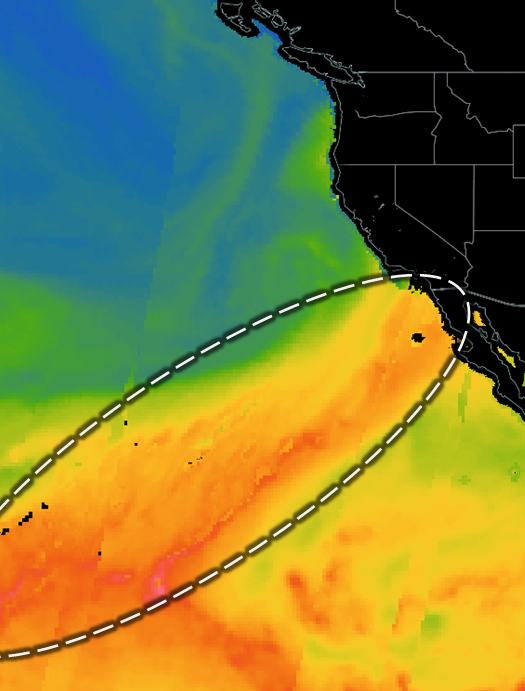
\includegraphics[width=0.4\textwidth]{images/ar}
        \end{tikzfigure}
    }
    \column{0.5}
    \block{Description of the figure}{\blindtext}
\end{columns}

\end{document}
